\chapter{Filtro activo de señal de campo}
\label{chap:senal-campo}

\section{Objetivos}
\label{sec:campo-objetivos}

\begin{itemize}
  \item Diseñar e implementar un filtro activo pasa bajos analógico para eliminar ruido de modo común y de alta
    frecuencia en líneas de instrumentación de gran longitud ($\SI{10}{\metre}$).
  \item Comprender el funcionamiento de un receptor diferencial y un convertidor tensión-corriente (V $\rightarrow$ I).
  \item Realizar la caracterización estática y dinámica del circuito mediante instrumental de laboratorio.
\end{itemize}

\section{Planteo del problema}
\label{sec:campo-planteo}

En un entorno industrial, un sensor transmite una variable de proceso mediante un bucle de
$\SI{4}{\milli\ampere}$ a $\SI{20}{\milli\ampere}$. El cable de interconexión recorre $\SI{10}{\metre}$ junto a
líneas de potencia, acoplando ruido de la red eléctrica ($\SI{50}{\hertz}$) y de conmutación de motores. Para que la
señal pueda ser procesada por la entrada analógica diferencial de corriente de un PLC, se diseña un módulo
intermedio de filtrado activo alimentado con la fuente industrial de $\SI{24}{\volt}$, compuesto por las tres etapas
en cascada de la figura~\ref{fig:diagrama-bloques}.

\begin{figure}[!ht]
  \centering
  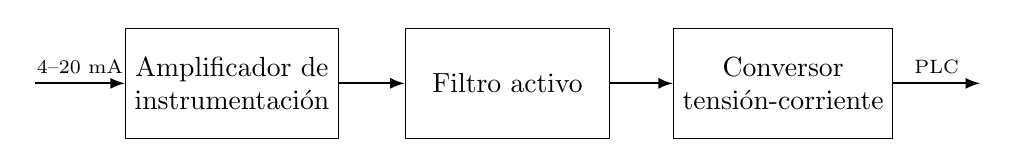
\begin{tikzpicture}[
    bloque/.style={draw, minimum width=2.6cm, minimum height=1.4cm, align=center},
    flecha/.style={->, >=latex, thick},
  ]
  \node[bloque] (e1) at (0,0) {Amplificador de\\instrumentación};
  \node[bloque] (e2) at (3.5,0) {Filtro activo};
  \node[bloque] (e3) at (7,0) {Conversor\\tensión-corriente};
  \draw[flecha] (-2.5,0) -- (e1) node[midway, above] {\scriptsize 4--20 mA};
  \draw[flecha] (e1) -- (e2);
  \draw[flecha] (e2) -- (e3);
  \draw[flecha] (e3) -- (9.5,0) node[midway, above] {\scriptsize PLC};
\end{tikzpicture}

  \caption{Diagrama en bloques del módulo de filtrado.}
  \label{fig:diagrama-bloques}
\end{figure}

\section{Especificaciones del circuito}
\label{sec:campo-especificaciones}

\subsection{Alimentación}
\label{subsec:campo-alimentacion}

Todo el módulo se alimenta con una fuente simple de $\SI{24}{\volt}$, sin tensión negativa. Por este motivo se
utiliza el LM324, cuyo rango de modo común de entrada incluye $\SI{0}{\volt}$ y cuya salida puede acercarse a masa.
El circuito completo requiere cinco amplificadores operacionales, por lo que se emplean dos integrados LM324:

\begin{itemize}
  \item U1A, U1B y U1C: etapa 1 (amplificador de instrumentación).
  \item U1D: etapa 2 (filtro Sallen-Key).
  \item U2A: etapa 3 (convertidor V $\rightarrow$ I). Las secciones U2B a U2D se conectan como seguidor con la entrada
    no inversora a masa.
\end{itemize}

El pin 4 de cada integrado se conecta a $\SI{+24}{\volt}$ y el pin 11 a GND, con un capacitor de desacople de
$\SI{100}{\nano\farad}$ lo más cerca posible de cada integrado.

% TODO: justificar brevemente por qué el TL084 no es apto con fuente simple (rango de entrada y excursión de salida).

\subsection{Etapa 1: receptor diferencial e instrumentación (I \texorpdfstring{$\rightarrow$}{->} V)}
\label{subsec:campo-etapa1}

La configuración de la etapa 1 se muestra en la figura~\ref{crkt:etapa1}. La resistencia de shunt flotante
$R_{shunt\_in} = \SI{250}{\ohm}$ convierte los $\SI{4}{\milli\ampere}$ a $\SI{20}{\milli\ampere}$ en una tensión
diferencial de $\SI{1}{\volt}$ a $\SI{5}{\volt}$. La resistencia $R_{CM} = \SI{1}{\mega\ohm}$ fija el modo común del
bucle flotante y provee el camino de polarización de las entradas. Los seguidores U1A y U1B evitan que la resistencia
de entrada del restador ($R_3 + R_4 = \SI{20}{\kilo\ohm}$) cargue al shunt, lo que produciría un error de ganancia de
$\SI{-1.23}{\percent}$. El restador U1C tiene ganancia unitaria con $R_3 = R_4 = R_5 = R_f = \SI{10}{\kilo\ohm}$
(tolerancia $\SI{1}{\percent}$ o mejor), de modo que

\begin{equation}
  V_{E1} = V_{(+)} - V_{(-)} = I_{in} \cdot R_{shunt\_in}
  \label{eq:ve1}
\end{equation}

\begin{figure}[!ht]
  \centering
  \begin{tikzpicture}[american, scale=0.9]
  % Operacionales
  \node[op amp] (u1a) at (5.2,3) {\scriptsize U1A};
  \node[op amp, noinv input up] (u1b) at (5.2,0) {\scriptsize U1B};
  \node[op amp] (u1c) at (10.6,1.5) {\scriptsize U1C};

  % Lazo (-) y (+)
  \draw (0,3.5) node[ocirc, label=left:{Lazo $(-)$}] {} to[short] (1.4,3.5) node[circ] {}
    to[short, -*] (3,3.5) -| (u1a.+);
  \draw (0,0) node[ocirc, label=left:{Lazo $(+)$}] {} to[short, i=$I_{in}$] (1.4,0) node[circ] {} -| (u1b.+);

  % Shunt y referencia de modo común
  \draw (1.4,3.5) to[R, l_=\shortstack{$R_{shunt\_in}$\\\SI{250}{\ohm}}] (1.4,0);
  \draw (3,3.5) to[R, l_=\shortstack{$R_{CM}$\\\SI{1}{\mega\ohm}}] (3,1.8) node[ground] {};

  % Seguidores
  \draw (u1a.out) -- ++(0.4,0) coordinate (ao);
  \draw (ao) -- ++(0,1.3) -| (u1a.-);
  \draw (u1b.out) -- ++(0.4,0) coordinate (bo);
  \draw (bo) -- ++(0,-1.3) -| (u1b.-);

  % Restador
  \draw (ao) node[circ] {} -- (ao |- u1c.-) to[R, l=\shortstack{$R_3$\\\SI{10}{\kilo\ohm}}] ($(u1c.-)+(-0.4,0)$)
    node[circ] (nm) {} -- (u1c.-);
  \draw (bo) node[circ] {} -- (bo |- u1c.+) to[R, l_=\shortstack{$R_4$\\\SI{10}{\kilo\ohm}}] ($(u1c.+)+(-0.4,0)$)
    node[circ] (np) {} -- (u1c.+);
  \draw (np) to[R, l=\shortstack{$R_5$\\\SI{10}{\kilo\ohm}}] ++(0,-2.6) node[ground] {};
  \draw (u1c.out) -- ++(0.4,0) coordinate (co) node[circ] {} -- ++(0,1.6) coordinate (ft);
  \draw (ft) to[R, l=$R_f$, a=\SI{10}{\kilo\ohm}] (ft -| nm) -- (nm);
  \draw (co) to[short, -o] ++(0.9,0) node[right, align=left] {$V_{E1}$\\\scriptsize 1--5 V};
\end{tikzpicture}

  \caption{Etapa 1: amplificador de instrumentación de ganancia unitaria.}
  \label{crkt:etapa1}
\end{figure}

\subsection{Etapa 3: convertidor tensión-corriente (V \texorpdfstring{$\rightarrow$}{->} I)}
\label{subsec:campo-etapa3}

La salida del filtro se reinyecta como corriente a la entrada analógica del PLC mediante una fuente de corriente tipo
sumidero con transistor NPN (figura~\ref{crkt:etapa3}). El operacional U2A fuerza la tensión de emisor a ser igual a
$V_{filtro}$, por lo que la corriente de salida resulta

\begin{equation}
  I_{out} = \alpha \, \frac{V_{filtro}}{R_{shunt\_out}} \approx \frac{V_{filtro}}{\SI{250}{\ohm}}
  \label{eq:iout}
\end{equation}

de modo que los $\SI{1}{\volt}$ a $\SI{5}{\volt}$ del filtro se convierten en $\SI{4}{\milli\ampere}$ a
$\SI{20}{\milli\ampere}$, donde $\alpha = \beta / (\beta + 1)$. Con $\beta \approx$ 100 a 200 el error por
corriente de base es de $\SI{-0.5}{\percent}$ a $\SI{-1}{\percent}$, y debe tenerse en cuenta en el análisis de
error de la caracterización estática.

\begin{figure}[!ht]
  \centering
  \begin{tikzpicture}[american]
  \node[op amp, noinv input up] (u2a) at (3,0) {\scriptsize U2A};
  \node[npn] (q1) at (7.5,0) {};
  \node[anchor=west] at ($(q1.C)+(0.1,-0.4)$) {\scriptsize Q1 (BC337)};

  % Entrada
  \draw (0,0.5) node[ocirc, label={[align=left]left:$V_{filtro}$\\\scriptsize 1--5 V}] {} -- (u2a.+);

  % Base
  \draw (u2a.out) to[R, l=$R_B$, a=\SI{1}{\kilo\ohm}] (q1.B);

  % Colector: carga (PLC) y +24 V
  \draw (q1.C) to[R, l=$R_{carga}$ (PLC), a=\SI{250}{\ohm}, i<=$I_{out}$] ++(0,2.8) node[vcc] {$\SI{+24}{\volt}$};

  % Emisor: shunt de salida y realimentación
  \draw (q1.E) -- ++(0,-0.5) node[circ] (fb) {} to[R, l=$R_{shunt\_out}$, a=\SI{250}{\ohm}] ++(0,-2.2)
    node[ground] {};
  \draw (fb) -- (1.3,0 |- fb) -- (1.3,0 |- u2a.-) -- (u2a.-);
\end{tikzpicture}

  \caption{Etapa 3: convertidor tensión-corriente.}
  \label{crkt:etapa3}
\end{figure}

% TODO: verificación de márgenes a 20 mA: caída en R_shunt_out y R_carga, V_CE y P_D del BC337.

\section{Diseño del filtro activo}
\label{sec:campo-diseno}

\subsection{Cálculo matemático}
\label{subsec:campo-calculo}

Se diseña un filtro pasa bajos Sallen-Key de segundo orden con aproximación Butterworth y ganancia unitaria en la
banda de paso, con frecuencia de corte $f_c = \SI{10}{\hertz}$ ($\SI{-3}{\decibel}$). La función de transferencia
buscada es

\begin{equation}
  H(s) = \frac{\omega_0^2}{s^2 + \dfrac{\omega_0}{Q} s + \omega_0^2}
  \qquad \text{con } Q = \frac{1}{\sqrt{2}} \text{ y } \omega_0 = 2 \pi f_c
  \label{eq:campo-hs}
\end{equation}

Para la topología Sallen-Key de ganancia unitaria de la figura~\ref{crkt:sk-unitario} se tiene

\begin{align*}
  \omega_0 &= \frac{1}{\sqrt{R_1 R_2 C_1 C_2}} \\
  Q &= \frac{\sqrt{R_1 R_2 C_1 C_2}}{C_2 \left( R_1 + R_2 \right)}
\end{align*}

% TODO: desarrollar el cálculo (p. ej. R_1 = R_2 = R, C_1 = 2 C_2 para Q = 1/sqrt(2)) y obtener los valores teóricos.

\begin{figure}[!ht]
  \centering
  \begin{tikzpicture}[american]
  \node[op amp, noinv input up] (oa) at (6,0) {\scriptsize U1D};

  \draw (0,0.5) node[ocirc, label=left:$V_{E1}$] {} to[R, l=$R_1$] (1.8,0.5) node[circ] (n1) {}
    to[R, l=$R_2$] (3.6,0.5) node[circ] (n2) {} -- (oa.+);
  \draw (n2) to[C, l_=$C_2$] ++(0,-2) node[ground] {};
  \draw (oa.out) -- ++(0.6,0) node[circ] (out) {} to[short, -o] ++(1,0) node[right] {$V_{filtro}$};
  \draw (n1) to[C, l=$C_1$] ++(0,2) -| (out);
  \draw (oa.-) -- ++(-0.5,0) |- ($(oa.south)+(0,-0.6)$) -| (out);
\end{tikzpicture}

  \caption{Etapa 2: filtro pasa bajos Sallen-Key de ganancia unitaria.}
  \label{crkt:sk-unitario}
\end{figure}

\subsection{Selección de componentes}
\label{subsec:campo-componentes}

% TODO: proponer valores comerciales normalizados (serie E12/E24), recalcular f_c y Q resultantes y justificar el
% uso de capacitores de poliéster o film (no electrolíticos).

\begin{table}[!ht]
  \centering
  \begin{tabular}{|l|c|c|}
    \hline
    Componente & Valor calculado & Valor comercial \\
    \hline
    $R_1$ & & \\
    $R_2$ & & \\
    $C_1$ & & \\
    $C_2$ & & \\
    \hline
  \end{tabular}
  \caption{Valores calculados y comerciales del filtro Sallen-Key.}
  \label{tab:campo-componentes}
\end{table}

\subsection{Simulación}
\label{subsec:campo-simulacion}

% TODO: simular el circuito completo (etapa 1 + filtro + etapa 3), incluir el diagrama de Bode y verificar
% analíticamente la atenuación a 50 Hz. Guardar el proyecto de simulación en sources/.

\section{Implementación}
\label{sec:campo-implementacion}

% TODO: descripción del armado en protoboard (dos LM324 + BC337/2N2222), fotos en pictures/, y cómo se generó la
% señal de 4-20 mA para la caracterización estática (fuente + resistencia/potenciómetro) y dinámica (generador +
% resistencia serie).

\section{Mediciones}
\label{sec:campo-mediciones}

\subsection{Caracterización estática (linealidad)}
\label{subsec:campo-estatica}

\begin{table}[!ht]
  \centering
  \begin{tabular}{|c|c|c|c|c|}
    \hline
    $I_{in}$ [mA] & $V_{E1}$ [V] & $V_{filtro}$ [V] & $I_{out}$ [mA] & Error [\%] \\
    \hline
    4  & & & & \\
    8  & & & & \\
    12 & & & & \\
    16 & & & & \\
    20 & & & & \\
    \hline
  \end{tabular}
  \caption{Caracterización estática del módulo.}
  \label{tab:campo-estatica}
\end{table}

% TODO: graficar la curva de transferencia I_out vs I_in y calcular el error porcentual por tolerancias.

\subsection{Caracterización dinámica (respuesta en frecuencia)}
\label{subsec:campo-dinamica}

\begin{table}[!ht]
  \centering
  \begin{tabular}{|c|c|c|c|}
    \hline
    $f$ [Hz] & $V_{in,pp}$ [V] & $V_{out,pp}$ [V] & $|H|$ [dB] \\
    \hline
    1   & & & \\
    2   & & & \\
    5   & & & \\
    10  & & & \\
    20  & & & \\
    50  & & & \\
    100 & & & \\
    \hline
  \end{tabular}
  \caption{Barrido en frecuencia del módulo (señal senoidal con offset de continua).}
  \label{tab:campo-dinamica}
\end{table}

% TODO: determinar la frecuencia de corte real a -3 dB y la atenuación exacta a 50 Hz; comparar con la simulación.
